\clearpage
\section{Postscript}

\vspace*{\fill}

\begin{example}
  \centering
  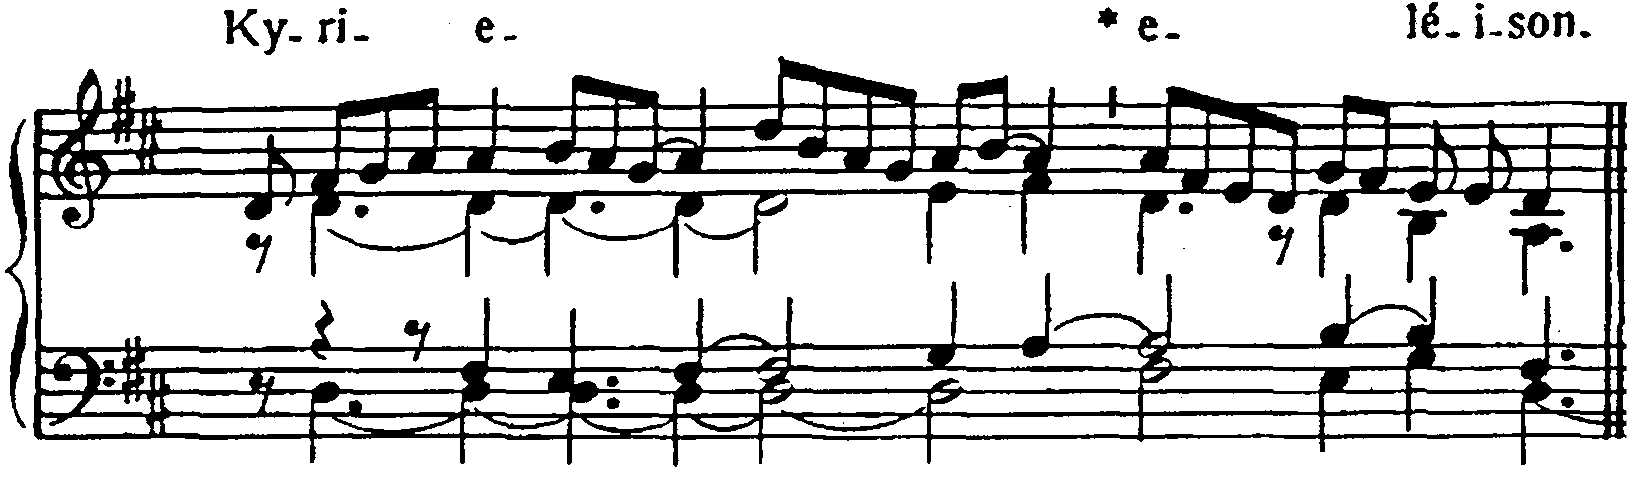
\includegraphics[width=.8\linewidth]{c/6/ex/portier_ictus.png}
  \caption{Portier, Additive method, 1981}
  \label{mus:portier_ictus_16}
\end{example}

\vspace*{\fill}

\begin{example}
  \centering
  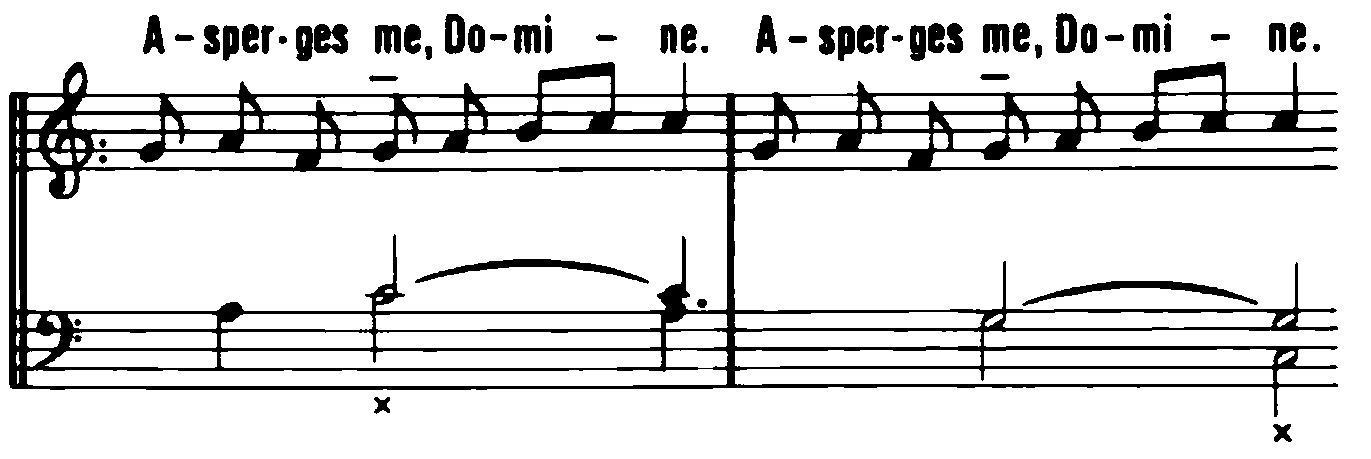
\includegraphics[width=.8\linewidth]{c/6/ex/migliavacca.png}
  \caption{Migliavacca, Restricted to notes present in chant, 1986}
  \label{mus:migliavacca}
\end{example}

\vspace*{\fill}

\newpage

\vspace*{\fill}

\begin{example}
  \centering
  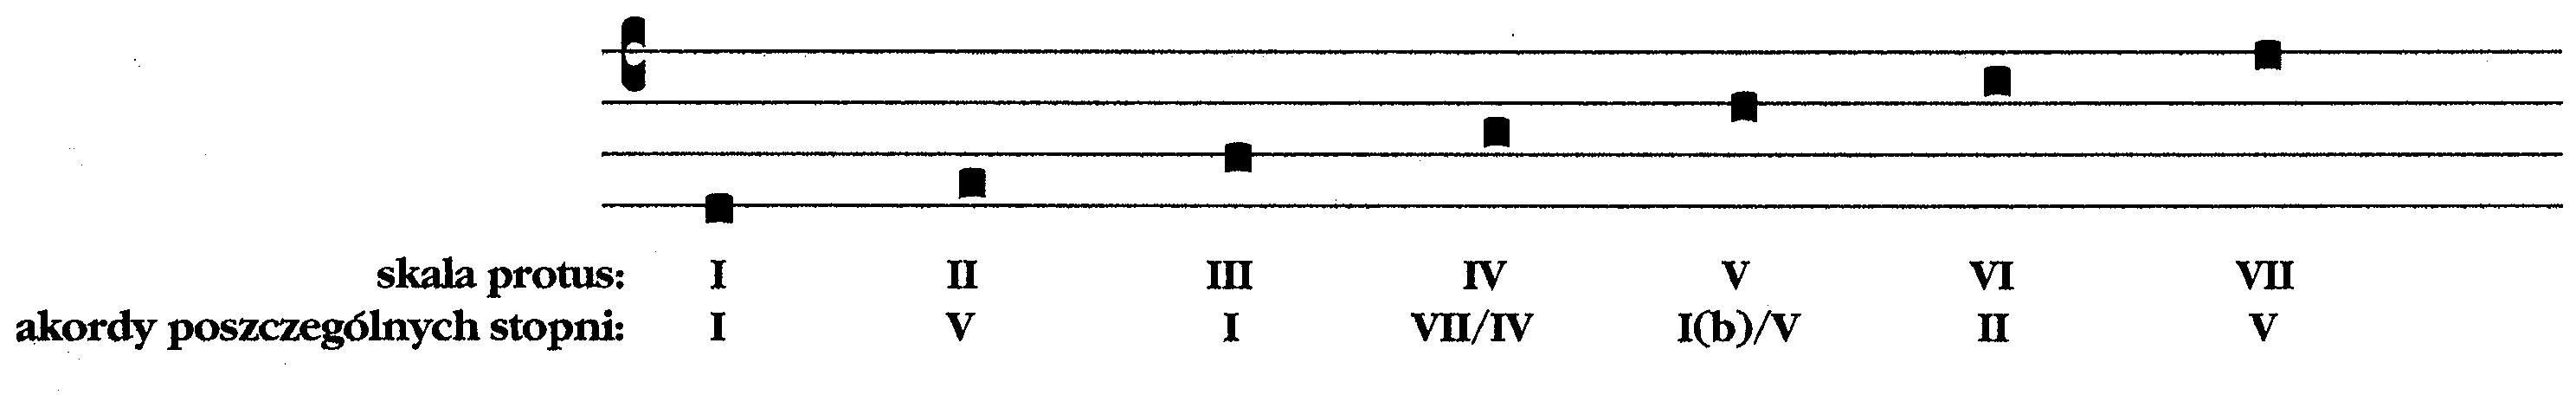
\includegraphics[width=.9\linewidth]{c/6/ex/bialowski_scale.png}
  \caption{Białowski, Protus scale degrees above chords, 2012}
  \label{mus:bialowski_scale}
\end{example}

\vspace*{\fill}

\begin{example}
  \centering
  \includegraphics[width=.9\linewidth]{c/6/ex/bialowski_harmonisation.png}
  \caption{Białowski, Protus harmonisation, 2012}
  \label{mus:bialowski_harmonisation}
\end{example}

\vspace*{\fill}

\newpage

\vspace*{\fill}

\begin{example}
  \centering
  \includegraphics[width=.9\linewidth]{c/4/ex/marier_analysis_148.png}
  \caption{Atwood, Analysis of Marier, 2014}
  \label{mus:marier_analysis}
\end{example}

\vspace*{\fill}
